%% This is file `elsarticle-template-1a-num.tex',
%%
%% Copyright 2009 Elsevier Ltd
%%
%% This file is part of the 'Elsarticle Bundle'.
%% ---------------------------------------------
%%
%% It may be distributed under the conditions of the LaTeX Project Public
%% License, either version 1.2 of this license or (at your option) any
%% later version.  The latest version of this license is in
%%    http://www.latex-project.org/lppl.txt
%% and version 1.2 or later is part of all distributions of LaTeX
%% version 1999/12/01 or later.
%%
%% The list of all files belonging to the 'Elsarticle Bundle' is
%% given in the file `manifest.txt'.
%%
%% Template article for Elsevier's document class `elsarticle'
%% with numbered style bibliographic references
%%
%% $Id: elsarticle-template-1a-num.tex 151 2009-10-08 05:18:25Z rishi $
%% $URL: http://lenova.river-valley.com/svn/elsbst/trunk/elsarticle-template-1a-num.tex $
%%
\documentclass[preprint,12pt]{elsarticle}

%% Use the option review to obtain double line spacing
%% \documentclass[preprint,review,12pt]{elsarticle}

%% Use the options 1p,twocolumn; 3p; 3p,twocolumn; 5p; or 5p,twocolumn
%% for a journal layout:
%% \documentclass[final,1p,times]{elsarticle}
%% \documentclass[final,1p,times,twocolumn]{elsarticle}
%% \documentclass[final,3p,times]{elsarticle}
%% \documentclass[final,3p,times,twocolumn]{elsarticle}
%% \documentclass[final,5p,times]{elsarticle}
%% \documentclass[final,5p,times,twocolumn]{elsarticle}

%% if you use PostScript figures in your article
%% use the graphics package for simple commands
%% \usepackage{graphics}
%% or use the graphicx package for more complicated commands
%% \usepackage{graphicx}
%% or use the epsfig package if you prefer to use the old commands
%% \usepackage{epsfig}

%% The amssymb package provides various useful mathematical symbols
\usepackage{amssymb}
%% The amsthm package provides extended theorem environments
%% \usepackage{amsthm}

%% The lineno packages adds line numbers. Start line numbering with
%% \begin{linenumbers}, end it with \end{linenumbers}. Or switch it on
%% for the whole article with \linenumbers after \end{frontmatter}.
%% \usepackage{lineno}

%% natbib.sty is loaded by default. However, natbib options can be
%% provided with \biboptions{...} command. Following options are
%% valid:

%%   round  -  round parentheses are used (default)
%%   square -  square brackets are used   [option]
%%   curly  -  curly braces are used      {option}
%%   angle  -  angle brackets are used    <option>
%%   semicolon  -  multiple citations separated by semi-colon
%%   colon  - same as semicolon, an earlier confusion
%%   comma  -  separated by comma
%%   numbers-  selects numerical citations
%%   super  -  numerical citations as superscripts
%%   sort   -  sorts multiple citations according to order in ref. list
%%   sort&compress   -  like sort, but also compresses numerical citations
%%   compress - compresses without sorting
%%
%% \biboptions{comma,round}

% \biboptions{}

%%%%%%%%%%%%%%%%%%%%%%%%%%%%%%%%%
% our packages and definitions: %
%%%%%%%%%%%%%%%%%%%%%%%%%%%%%%%%%
\usepackage{url} 
\usepackage{color}
% \usepackage{dsfont}

\newcommand{\TODO}[1]{{\color{red}TODO: #1}}
\newcommand{\TODON}[1]{{\color{blue}TODO: #1}}
\newcommand{\COMMENTD}[1]{{\color{green}Dimo: #1}}
\newcommand{\COMMENTN}[1]{{\color{green}Nora: #1}}


\journal{DAM}

\begin{document}

\begin{frontmatter}

%% Title, authors and addresses

%% use the tnoteref command within \title for footnotes;
%% use the tnotetext command for the associated footnote;
%% use the fnref command within \author or \address for footnotes;
%% use the fntext command for the associated footnote;
%% use the corref command within \author for corresponding author footnotes;
%% use the cortext command for the associated footnote;
%% use the ead command for the email address,
%% and the form \ead[url] for the home page:
%%
%% \title{Title\tnoteref{label1}}
%% \tnotetext[label1]{}
%% \author{Name\corref{cor1}\fnref{label2}}
%% \ead{email address}
%% \ead[url]{home page}
%% \fntext[label2]{}
%% \cortext[cor1]{}
%% \address{Address\fnref{label3}}
%% \fntext[label3]{}

\title{An Evolutionary Algorithm for the Multiobjective Risk-Equity Constrained Routing Problem}

%% use optional labels to link authors explicitly to addresses:
%% \author[label1,label2]{<author name>}
%% \address[label1]{<address>}
%% \address[label2]{<address>}

\author{Dimo Brockhoff}
\address{INRIA Lille - Nord Europe, DOLPHIN team, 59650 Villeneuve d'Ascq, France\\
{\upshape \url{dimo.brockhoff@inria.fr}}}

\author{Nora Touati-Moungla}
\address{Laboratoire d'Informatique, \'{E}cole Polytechnique, 91128 Palaiseau Cedex, France\\
{\upshape \url{touati@lix.polytechnique.fr}}}



\begin{abstract}


\end{abstract}

\begin{keyword}
Evolutionary multiobjective optimization, Transportation of hazardous materials, Risk equity, Shortest Paths. 
\end{keyword}

\end{frontmatter}
\section{Introduction}

The transportation of hazardous materials ({\em hazmat} from now on) has received a large interest in recent years, which results from the increase in public awareness of the dangers of hazmats and the enormous amount of hazmats being transported \cite{CAR08}. The main target of this problem is to select routes from a given origin-destination pair of nodes such that the risk for the surrounding population and the environment is minimized---without producing excessive economic costs. 
%
When solving such a problem by minimizing both cost and the total risk, typically several vehicles share the same (short) routes which results in high risks associated to regions surrounding these paths whereas other regions are not affected. In this case, one may wish to distribute the risk in an equitable way over the population and the environment. Several studies consider this additional minimization of the equity risk, but most of them consist of a \emph{single} origin-destination hazmat routing for a specific hazmat, transport mode and vehicle type (see for example \cite{AKG02, CAR08}).
% 
% 
% and can be classified into the \textit{resolution-equity-based methods} and the \textit{model-equity-based methods}. In resolution-equity-based methods, the equity constraints are taken into account only indirectly via a dissimilarity index between paths which is to be maximized \cite{JOH92, LOM93, KUB97, AKG02}. Model-equity-based methods, on the other hand, formalize the risk equity as constraints directly within the model. In \cite{GOP90a, GOP90b}, for example, the authors propose an equity shortest path model that minimizes the total risk of travel while the difference between the risks imposed on any two arbitrary zones does not exceed a given threshold.
%
A more realistic \emph{multi}-commodity flow model was proposed in \citep{CAR08} where each commodity is considered as one hazmat type. The objective function is formulated as the sum of the economical cost and the cost related to the consequences of an incident for each material. To deal with risk equity, the costs are defined as functions of the flow traversing the arcs which imposes an increase of the arc's cost and risk when the number of vehicles transporting a given material increases on the arc.

The majority of all hazmat routing studies deal with a single-objective scenario although the problem itself is multiobjective in nature and it is important to study the trade-offs among the objectives. Evolutionary Multiobjective Optimization (EMO) algorithms are able to compute a set of solutions showing these trade-offs within a single algorithm run which is the reason why we propose to use them for the problem of hazmat routing in this study (Sec.~\ref{S_MEO}). Before, we formalize the routing of hazmat problem with three objectives (minimize total routing cost, total routing risk {\em and} risk equity) as a multicommodity flow model as in \cite{CAR08} since this model is the most realistic one permitting to manage several hazmat types simultaneously (Sec.~\ref{S_RECRP}).



% see for example \cite{CAR08, cgr2007, gkbk1990, za2004}, but all problem formulations include the equity risk as constraints and not as an additional objective. \citet{gian1998} on the other hand considers the equity risk as separate objective but uses a weighted sum to aggregate his four objectives into a single-objective problem. The main reason why, to the best of our knowledge, no study considered a fully multiobjective model with the equity risk as objective might be the resulting non-linearity of the problem which make classical optimization algorithms such as branch-and-cut \TODON{equity is an objective in \cite{{gian1998}} ... We solve the broblem with a branch and price algorithm because the model is a multicommodity flow model, and this model is the more adapted one for this problem because it permit to manage simultaneously many hazmat types. The min-max formulation of the objective is easily linearized. I give you the major axes of the work: (1) Solve the presented problem (optimize cost, risk and equity) (2) what are models and resolution methods proposed in the litterature (3) what is the model retained and why (in our case, the multicommodity model) (4) how to handle equity with this model ? (5) how to solve it ? (branch and price is adapted for these models, but can not hadle many objectives $->$ evolutionnary algorithms) } infeasible and led us to our choice of proposing an evolutionary multiobjective algorithm as heuristic here.

%The computation of routes with a fairly distributed risk consists in generating dissimilar origin-destination paths, i.e paths which relatively don't impact the same zones. Solution approaches 

%Section~\ref{S_RECRP} defines the problem of transporting hazardous materials with equity risk as a three-objective optimization problem with the minimization of the total routing cost, of the total routing risk {\em and} of the risk equity as the objectives---the latter broadly defined as the risk shared by a set of regions that compose the geographical area under consideration. Based on this formulation, Sec.~\ref{S_MEO} presents an evolutionary multiobjective optimization algorithm before Sec.~\ref{S_FW} concludes the abstract.


%In \cite{CAR08} was proposed a multi-commodity flow model for this problem, where each commodity is considered as one hazmat type. To deal with risk equity, the costs are defined as functions of the flow traversing the arcs, this imposes an increase of the arc's cost and risk when the number of vehicles transporting a given material increases on the arc. The major drawback of this model is that it can lead to the saturation of the arcs of shortest paths and, therefore, does not guarantee the equity target. 

%In \cite{BEL10}, the authors consider a similar model but with additional equity constraints and objectives. The objective is the minimization of the maximum risk equity imposed on the population and the environment and the model is solved using a pranch-and-price algorithm. 

%As hazmat routing is multiobjective in nature, we introduce in this work a multiobjective version of this problem. Our goal is the minimization of the total routing cost, of the total routing risk {\em and} of the risk equity, the latter broadly defined as the risk shared by a set of regions that compose the geographical area under consideration. 

%This paper is organized as follows. We describe the problem in section \ref{S_RECRP}, we give its mathematical formulation in section \ref{S_AOM}, in section \ref{S_MEO} we show how multiobjective evolutionary methods can be applied to this problem and in section \ref{S_FW} we exopse our further work.


%%%%%%%%%%%%%%%%%%%%%%%%%%%%%%%%%%%%%%%%%%%%%%%%%%%%%%%%%%%%%%%%%%%%%%%%%%%%%%%%%%%%%%%%%%%%
\section{The multiobjective risk-equity constrained routing problem}
\label{S_RECRP}

Let the transportation network be represented as a directed graph $G = (N, A)$, with $N$ being the set of nodes and $A$ the set of arcs. Let $C$ be the set of commodities, given as a set of point-to-point demands to transport a certain amount of hazmats. For any commodity $c\in C$, let $s^c$ and $t^c$ be the source node and the destination node respectively, and let $d^c$ be the amount of hazmat to be shipped from $s^c$ to $t^c$. We assume that the risk is computed on each arc of the network and is proportional to the arc length and the population density around this arc, and we define $r_{ij}^c$ as the risk imposed on the population when the arc $(i, j) \in A$ is used for the transportation of one unit of hazardous materials of type $c$. With each arc $(i,j) \in A$ a cost $c_{ij}$ is associated, equivalent to the length of arc $(i,j)$.

\subsection{Multiple objective functions}
\label{SS_MOF}


The problem of transporting hazmat is multiobjective in nature: one usually wants to minimize the \textit{total cost} of transportation, the \textit{total risk} of transportation and the {\em distributed risk}, which can be defined as a measure of risk that is shared among different arcs or different paths. 

\subsection{An optimization model}
\label{SS_AOM}

We introduce a flow variable $f_{ij}^c$ defining the portion of commodity $c$ being transported on arc $(i,j)$. These variables are subject to flow conservation constraints:

$$\sum_{j \in \delta^+(i)} f_{ij}^c -  \sum_{j \in \delta^-(i)} f_{ji}^c = b_i^c, \forall i \in N,  c \in  C$$

where $\delta^-(i)$ and $\delta^+(i)$ are the forward and backward star of $i$, i.e., $\delta^-(i) = \{j \in N: (j,i)\in A\}$ and $\delta^+(i) = \{j \in N: (i,j)\in A\}$, and $b_i^c=\left\{
\begin{array}{rl}
                     1 & \textrm{ if } i=s^c\\
                    -1 & \textrm{ if } i=t^c\\
                     0 & \textrm{ otherwise.}\\
\end{array}\right.$

The first objective is a cost function given as follows:

$$\min \sum_{c \in C} \sum_{(i,j) \in A} c_{ij} f_{ij}^c$$


The second objective is the minimization of the total risk

$$
\min \sum_{c \in C} \sum_{(i,j) \in A} r_{ij}^c f_{ij}^c
$$

We define the risk $w_{ij}$ imposed on the population around the arc $(i,j)$ as a linear combination of the flow variables: 

$$w_{ij} = \sum_{c \in C} r_{ij}^c f_{ij}^c$$

and add a new variable $z = \max_{(i,j) \in A} w_{ij}$, which therefore is subject to the constraints

$$
z \geq \sum_{c \in C} r_{ij}^c f_{ij}^c, \forall (i,j) \in A
$$

% We define the risk $w_p$ imposed on the population around the path $p$ as a linear combination of the flow variables: 
% 
% $$w_p = \sum_{c \in C} \sum_{(i,j) \in p} r_{ij}^c f_{ij}^c$$
% 
% and add a new variable $y = \max_{p \in \mathcal{P}} w_p$, which therefore is subject to the constraints
% 
% $$
% y \geq \sum_{c \in C} \sum_{(i,j) \in p} r_{ij}^c f_{ij}^c, \forall p \in \mathcal{P}
% $$
% 
% where $\mathcal{P}$ is the set of paths.



% 
% 
% 
% The third and fourth objectives will then be:
% $$\min \max_{(i,j)\in A} r_{ij} f_{ij}^c$$, and 
% $$\min \max_{p \in \mathcal{P}} \sum_{(i,j) \in p} r_{ij} f_{ij} $$ 
% 
% where 

% We introduce the integer variable $y_{ij}^c$ for the number of trucks that use arc $(i,j)$ for transporting commodity $c$. We assume a fixed number of trucks and that all trucks have the same load. 



The proposed model is defined as follows:
\begin{eqnarray}
   \min  &  \sum_{c \in C} \sum_{(i,j) \in A} c_{ij} f_{ij}^c & \label{eq:obj1}\\
   \min  &  \sum_{c \in C} \sum_{(i,j) \in A} r_{ij}^c f_{ij}^c & \label{eq:obj2}\\
   \min  & z & \label{eq:obj3}\\
   %\min  & y & \label{eq:obj4}\\
    s.t. & \sum_{j \in \delta^+(i)} f_{ij}^c -  \sum_{j \in \delta^-(i)} f_{ji}^c = d_i^c\quad         & \forall i \in N,  c \in  C \label{eq:flow} \\
    & z \geq \sum_{c \in C} r_{ij}^c f_{ij}^c & \forall (i,j) \in A \\
%     & y \geq \sum_{c \in C} \sum_{(i,j) \in p} r_{ij}^c f_{ij}^c & \forall p \in \mathcal{P}
%          & y_{ij}^c \in \{0, 1, 2, \ldots\}                                                            & \forall (i,j)\in A, c\in C\label{eq:integerY}.
\end{eqnarray}

% The first objective in (\ref{eq:obj1}) is a cost function and is to be minimized. The second objective, given by (\ref{eq:obj2}), minimizes the total risk on all regions and objective (\ref{eq:obj3}) minimizes the maximum risk imposed on all regions. Constraints (\ref{eq:flow}) are conservation constraints, where $\delta^-(i) = \{j \in N: (j,i)\in A\}$ and $\delta^+(i) = \{j \in N: (i,j)\in A\}$ are the direct successors and predecessors of node $i$, and $q_i^c=V^c$ if  $i=s^c$, $q_i^c=-V^c$ if  $i=t^c$ and $q_i^c=0$ otherwise.

% \begin{Rq}
% The number of constaints $nbC = |N| + |A| + |\mathcal{P}|$ is exponontial, so the classical optimization softwares such as CPLEX can not be used.
% \end{Rq}


\section{Evolutionary multiobjective optimization}
\label{S_MEO}
Evolutionary algorithms (EAs) and Evolutionary Multiobjective Optimization (EMO) algorithms in particular are general-purpose randomized search heuristics and as such well suited for problems where the objective function(s) can be highly non-linear, noisy, or even given only implicitly, e.g., by expensive simulations \citep{deb2001a,cvl2007a}. Since the third objective in the above problem formulation is nonlinear, we propose to use an EMO algorithm for the multiobjective risk-equity constrained routing problem here. Our EMO algorithm follows the standard iterative/generational cycle of an EA of mating selection, variation, objective function evaluation, and environmental selection and is build upon the state-of-the-art selection scheme in HypE \citep{bz2011a} as implemented in the PISA platform \citep{bltz2003a}. The variation operators as well as the representation of the solutions, however, have to be adapted to the problem at hand in the following way in order to fulfill the problem's constraints at all times\footnote{The source code of the corresponding PISA hazmat variator is going to be available on the official PISA web page \url{http://www.tik.ee.ethz.ch/pisa/} and until then can be downloaded on the preliminary web page \url{http://researchers.lille.inria.fr/~brockhof/downloads/hazmatvariator20111110.zip}}.

\subsection{Representation}
We choose a variable length representation as it has been theoretically shown to be a good choice for multiobjective shortest paths problems \citep{horo2009a}: A solution is thereby represented by a list of paths of variable lengths with one path per truck. We decided to consider a fixed amount of trucks for each commodity and therefore a fixed number of paths through the network although, in principle, the number of trucks could change during the algorithm run if an appropriate mutation operator is designed. The left hand side of Fig.~\ref{fig:paths} shows an exemplary solution with two trucks for commodity 1 and one truck for commodity 2.

In order to have every variable length path represent an uninterrupted path from source to destination at any time (see the constraints in (\ref{eq:flow})), we ensure all paths to always start with the source $s^c$ for the corresponding commodity $c$, ensure during initialization and variation that all neighbored vertices in the path are connected by an arc (see Sec.~\ref{sec:init} and \ref{sec:variation}), and complete each path by the shortest path between the path's actual end node and the commodity's destination node $t^c$. The right hand side of Fig.~\ref{fig:paths} shows the entire source--destination paths corresponding to the representation in the left part of the figure. 

\begin{figure}%

\includegraphics[width=\columnwidth]{figs/truckpaths}%
\caption{\label{fig:paths} Illustration of the variable-length representation of a solution (left) with its two paths for commodity 1 and one path for commodity 2 in opposition to the resulting full source--destination paths where the last part is the shortest path between the variable-length path's end node and the destination node for this commodity (right). The source and destination nodes for commodity 1 are 0 and 6 and for the second commodity the source is node 1 and the destination is node 7. The smaller numbers along the arcs depict the costs.}
\end{figure}


\subsection{Initialization}\label{sec:init}
\begin{itemize}
	\item Typically, the initialization of EAs is random (often uniformly at random in the search space)
	\item here, a uniform initialization is more complicated if not impossible due to the non-standard search space (how do you define a uniform probability distribution on paths thorough a network?)
	\item hence, a simple random initialization procedure is proposed: explain idea
	\item in addition, we have the opportunity to use the shortest paths within the network to have another initialization: all truck paths are initialized with the shortest path, i.e., in the representation, only the source node is chosen in the beginning
	\item advantage: we know that this initialization immediatly gives us a (weak) Pareto-optimal point, namely the one with the smallest cost (objective 
\end{itemize}

Initially, we start with a single solution where the paths $p$ for all trucks are empty ($p=(s^c)$). This corresponds to the situation where all trucks choose the shortest $s^c$--$t^c$ path for their assigned commodity---implying the smallest possible overall cost but a high risk along the used route(s). Nevertheless, the initial solution is already Pareto-optimal and is expected to be a good starting point for the algorithm.

\subsection{Variation}\label{sec:variation}
As mutation operator, we suggest to shorten or lengthen the path of one or several trucks. In order to generate a new solution $s'$ from $s$, for each truck path, we draw a binary value $b\in\{0,1\}$ uniformly at random and create the new path $p'$ from the old one $p=(v_1=s^c,v_2,\ldots, v_l)$ as in \citep{horo2009a}:
\begin{itemize}
	\item if $b = 0$ and $l=:\textnormal{length}(p)\geq 2$, set $p' = (s^c, \ldots, v_{l-1})$	
	\item if $b = 1$ and $|V_{\textnormal{\scriptsize rem}}=\{v \in V \,|\, (v_{l}, v) \in A\}| \neq\emptyset$, choose $v_{l+1}$ from $V_{\textnormal{\scriptsize rem}}$ uniformly at random and set $p' = (v_0, \ldots, v_l, v_{l+1})$.
	\item otherwise, use the same path $p$ also in the new solution $s'$.
\end{itemize}

\subsection{Implementation in PISA}
The proposed algorithm has been implemented within the multiobjective optimization framework PISA \citep{bltz2003a} and is going to be made available via the official PISA web page\footnote{Until the source code is available via the PISA web page \url{http://www.tik.ee.ethz.ch/pisa/}, we make it temporarily available at \url{http://researchers.lille.inria.fr/~brockhof/downloads/hazmatvariator20111110.zip} as supplementary material for the review process.}.

\section{Experimental analysis}

We concentrated our analysis on a real-world case study \cite{bianco09}. We considered the road network of the Lazio region (located in the middle of Italy), and, in particular, its main transport roads. The network is composed of 311 nodes and 441 links. The risk $r_{ij}^c, \forall (i,j) \in A, c \in C$ is evaluated as the societal risk computed as the number of people living inside the exposure zone around link $(i,j)$ (whose size depends on the hazmat type $c$ times the accident probability involving the vehicle. We considered from 2 to 10 origin-destination pairs on the network, each one associated with a number of commodities ranging from 1 to 3, for an overall number of shipments (commodities) between 2 and 30 (we recall that in our model each commodity is associated with one origin-destination pair). With each one of the latter scenarios we associated 10 instances; each instance has been generated by assigning uniformly at random a demand from 100 to 1000 tons to each shipment.


\subsection{Random Initialization Versus Cost-Optimal Initialization}

\begin{figure}%
	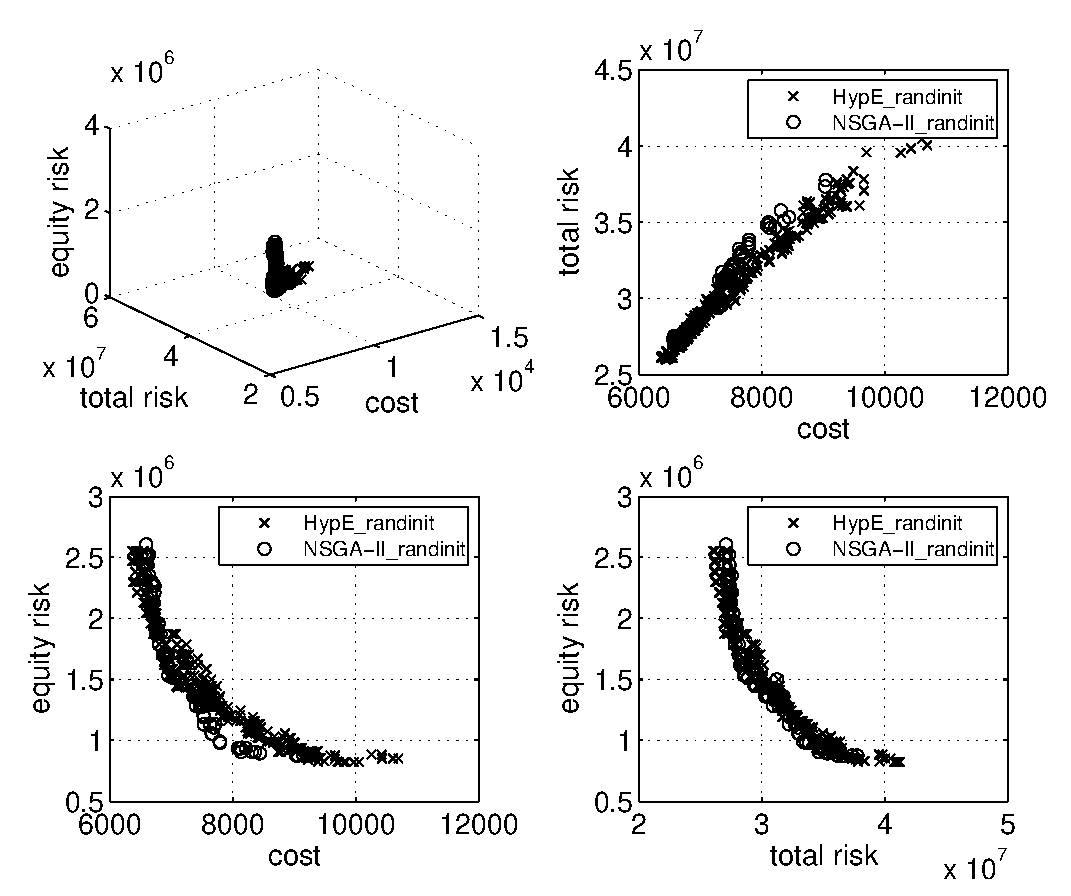
\includegraphics[width=\columnwidth]{../experiments/randVsCost/allsolutions.eps}%
	\caption{\label{fig:allsolutions} Comparison between the random initialization (circles) and the cost-optimal one (crosses). Shown are the populations of 10 independent HypE runs after 1000 generations for all three objectives (top left) and each combination of two objectives.}
\end{figure}

\begin{figure}%
	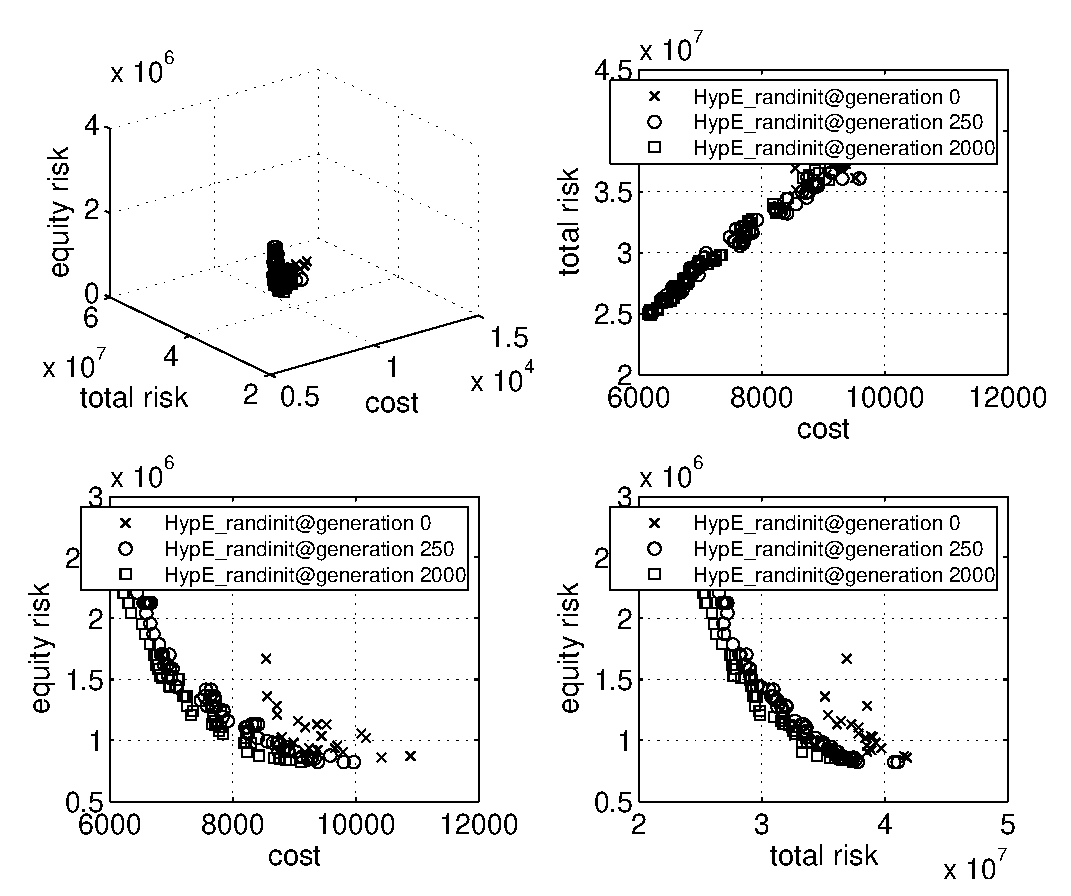
\includegraphics[width=\columnwidth]{../experiments/randVsCost/onlynondominated.eps}%
	\caption{\label{fig:onlynondominated} Comparison between the random initialization (circles) and the cost-optimal one (crosses). Shown are only the non-dominated solutions in the final populations of 10 independent HypE runs after 1000 generations.}
\end{figure}


\subsection{Comparison With An Exact Algorithm for the Two Linear Objectives}
\TODO{add plots and describe what we compare (efficient cost/risk paths multiplied by the number of trucks); result: EA is better}


\section{Conclusions}
\label{S_FW}
The transportation of hazmats is an important optimization problem in the field of sustainable development and in particular the equitable distribution of risks is of high interest. Within this study, we formalize this transportation problem as the minimization of three objectives and propose to use an evolutionary algorithm to cope with the non-linear equity risk objective.

The third objective function of our problem can be rewritten by minimizing the additional variable $z$ as third objective and adding the constraints $\forall q \in Q: z \geq \sum_{c \in C} \sum_{(i,j) \in A} r_{ij}^{cq} f_{ij}^c$. Although this equivalent formulation makes the problem linear (with additional linear constraints), classical algorithms are expected to have difficulties with this formulation as well and our algorithm is supposed to be more efficient in the current formulation due to the fewer number of constraints. Note that, for the moment, the proposed EMO algorithm exists on paper only and an actual implementation has to prove in the future which additional algorithm components (such as problem-specific initialization, recombination operators, or other exact optimization (sub-)procedures) are necessary to generate solutions of sufficient quality and whether adaptively changing the number and capacity of trucks is beneficial.




% The transportation of hazmats is an important optimization problem in the field of sustainable development and in particular the equitable distribution of risks is of high interest. 

% In this study, we formalize transportation of hazmats problem as the minimization of three objectives and propose to use an evolutionary algorithm since many exact optimization procedures have difficulties with the non-linear equity risk objective. Note that our problem formulation can be rewritten by minimizing the additional variable $z$ as third objective and adding the constraints $\forall q \in Q: z \geq \sum_{c \in C} \sum_{(i,j) \in A} r_{ij}^{cq} f_{ij}^c$ \COMMENTD{this has to be adapted according to the new problem formulation}. Although this equivalent formulation makes the problem linear (with additional non-linear constraints), classical algorithms are expected to have difficulties with this formulation as well and the EMO algorithm is supposed to be more efficient in the current formulation due to the fewer number of constraints.
% 
% Note also that, for the moment, the proposed EMO algorithm only exists as a gedankenexperiment and an actual implementation has to prove in the future which additional algorithm components (such as problem-specific initialization, recombination operators, or other exact optimization (sub-)procedures) are necessary to improve the quality of the found solutions to a sufficient level.


% 
 \bibliographystyle{plainnat}
 \footnotesize
% \bibliography{hazmat}

\begin{thebibliography}{00}
% \providecommand{\natexlab}[1]{#1}
% \providecommand{\url}[1]{\texttt{#1}}
% \expandafter\ifx\csname urlstyle\endcsname\relax
%   \providecommand{\doi}[1]{doi: #1}\else
%   \providecommand{\doi}{doi: \begingroup \urlstyle{rm}\Url}\fi

\bibitem[Akgun et~al.(2003)Akgun, Erkut, and Batta]{AKG02}
V. Akgun, E. Erkut and R. Batta, 
On finding dissimilar paths, 
European Journal of Operational Research 121(2):232-246, 2000.

\bibitem[Bader and Zitzler(2011)]{bz2011a}
J.~Bader and E.~Zitzler.
\newblock Hype: An algorithm for fast hypervolume-based many-objective
  optimization.
\newblock \emph{Evolutionary Computation}, 19\penalty0 (1):\penalty0 45�--76,
  2011.

\bibitem[Bleuler et~al.(2003)Bleuler, Laumanns, Thiele, and Zitzler]{bltz2003a}
S.~Bleuler, M.~Laumanns, L.~Thiele, and E.~Zitzler.
\newblock PISA---a platform and programming language independent interface for
  search algorithms.
\newblock In \emph{Evolutionary
  Multi-Criterion Optimization {(EMO~2003)}}, pages
  494--508, 2003. Springer.

\bibitem[Caramia et~al.(2008)Caramia and Dell'Omo]{CAR08}
M. Caramia and P. Dell'Olmo, 
Multiobjective management in freight logistics: increasing capacity, service level and safety with optimization algorithms,
Springer London Ltd, 2008.

\bibitem[{Coello Coello} et~al.(2007){Coello Coello}, {Lamont}, and {Van
  Veldhuizen}]{cvl2007a}
C.~A. {Coello Coello}, G.~B. {Lamont}, and D.~A. {Van Veldhuizen}.
\newblock \emph{Evolutionary Algorithms for Solving Multi-Objective Problems}.
\newblock Springer, 2007.

\bibitem[Deb(2001)]{deb2001a}
K.~Deb.
\newblock \emph{Multi-Objective Optimization Using Evolutionary Algorithms}.
\newblock Wiley, Chichester, UK, 2001.

\bibitem[Horoba(2009)]{horo2009a}
C.~Horoba.
\newblock Analysis of a simple evolutionary algorithm for the multiobjective
  shortest path problem.
\newblock In \emph{Foundations of Genetic Algorithms {(FOGA 2009)}}, pages
  113--120. ACM, 2009. 

\bibitem[bianco(2009)]{bianco09}
L. Bianco and M. Caramia and S. Giordani.
\newblock A bilevel flow model for hazmat transportation network design.
\newblock Transportation research. Part C, Emerging technologies, 17(2):175--196, 2009.



% \bibitem{GOP90b}
% R. Gopalan, K.S. Kolluri, R. Batta and M.H. Karwan, 
% Modeling equity of risk in the transportation of hazardous materials, 
% Operations Research, 38(6):961-973, 1990.
% 
% \bibitem{KUB97}
% M. Kuby, X. Zhongyi and X. Xiaodong, 
% A minimax method for finding the $k$ best differentiated paths, 
% Geographical Analysis 29(4):298-313, 1997.

% \bibitem{LOM93}
% K. Lombard and R.L. Church, 
% The gateway shortest path problem: Generating alternative routes for a corridor location problem, 
% Geographical Systems, 1:25-45, 1993.

\end{thebibliography}


\end{document}

%%
%% End of file `elsarticle-template-1a-num.tex'.
